\documentclass[a4paper,11pt,dvipdfmx]{ujarticle}

\usepackage{graphicx}
\usepackage{url}

\input{layout}

\title{日本におけるデジタル化の状況}

\author{G584052025 オウニンキ}

\begin{document}

\maketitle


\section{ブロードバンドの整備状況}

OECDによるブロードバンド回線の普及に関する調査\cite{oecd}によると、図\ref{fig:加入者}に示すように、日本におけ
る100人あたりの光ファイバー回線の加入者数は29.0で、韓国、スウェーデン、ノルウェーに続いて第
4位になっている。

%  参考文献の参照: \cite{}
%  図番号の参照: \ref{}

% 文献データベースのキーワードは oecd と imd

\begin{figure}[htbp]
    \centering
    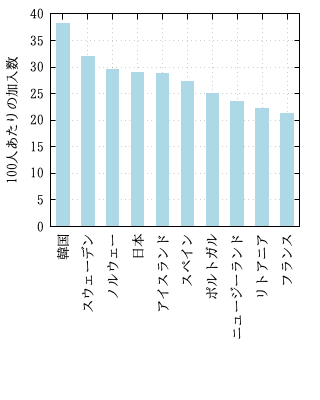
\includegraphics{fig11.png}
    \caption{光ファイバー回線の加入者(100人あたり)}\label{fig:加入者}
\end{figure}


\section{デジタル競争力ランキング}

国際経営開発研究所(IMD)の調査\cite{imd}によると、
表\ref{tbl:競争力ランキング}にすように、
日本のデジタル競争力のランキングは調査対象の64カ国中、総合で28位、知識分野で25位となっている。

% 表の挿入
\begin{table}[htbp]
    \centering
    \caption{デジタル競争力ランキング(64カ国中)}\label{tbl:競争力ランキング}
    \begin{tabular}{|c|c|c|}
        \hline
        国 & 総合 & 知識 \\
        \hline
        米国 & 1位 & 3位 \\
        \hline
        香港 & 2位 & 5位 \\
        \hline
        スウェーデン & 3位 & 2位 \\
        \hline
        デンマーク & 4位 & 8位 \\
        \hline
        シンガポール & 5位 & 4位 \\
        \hline
        \hline
        韓国 & 12位 & 15位 \\
        \hline
        中国 & 15位 & 6位 \\
        \hline
        \hline
        日本 & 28位 & 25位 \\
        \hline
    \end{tabular}
\end{table}
% で囲み

% 考察
\section{考察}

日本におけるブロードバンドの整備状況を見ると、
普段の利用状況について尋ねた結果は次のようになっている.
\begin{itemize}
    \item  光ファイバー回線の加入者数は100人あたり29.0人
    \item  韓国、スウェーデン、ノルウェーに次いで第4位となっている
    \item  日本は総合で28位、知識分野では25位
\end{itemize}
% を使って箇条書きで記述する
このことから、日本は通信インフラの整備は進んでいるものの、
デジタル技術の活用や人材育成といった面では、他国に比べて課題があることがわかる。
% ここに参考文献が入る

\bibliographystyle{junsrt}
\bibliography{exercise.bib}

\end{document}